% !BIB TS-program = bibtex

%-----------------------------------------------------------------------------
%
% Conference CCC - http://www.utb.edu.co/13ccc
% Page limit: 15 pages 
% Submission deadline: 
%			Abstract: May 8st
%			Full paper: May 24th
% Notification: June 30th
% Revisions: July 10th 
%
%-----------------------------------------------------------------------------

\documentclass[draft]{llncs}


%---- PACKAGES
%\usepackage{todonotes}
\usepackage{amssymb}
\usepackage{hyperref}
\usepackage[plain]{fancyref}
\usepackage{ifdraft}
%\usepackage{subcaption}
\let\labelindent\relax
\usepackage[inline]{enumitem}
\usepackage{xcolor}
\usepackage[final]{graphicx}
\usepackage{xspace}
\usepackage[final]{listings}
\usepackage{acronym}
\usepackage{url}
\usepackage{amsmath}
\usepackage{amssymb}
\usepackage[square,numbers,sectionbib]{natbib}
\bibliographystyle{abbrvnat}

\usepackage{etoolbox}
\makeatletter
\patchcmd{\@makecaption}
  {\scshape}
  {}
  {}
  {}
\patchcmd{\@makecaption}
  {\\}
  {.\ }
  {}
  {}
\makeatother

%\let\refsection\relax
%\usepackage
%  [backend=biber,
%   style=trad-abbrv,
%   maxnames=5,
%   firstinits=true,
%   hyperref=true,
%   natbib=true,
%   url=false,
%   doi=false,
%   defernumbers]{biblatex}
%
%
%----[ Biber ]----
%\addbibresource[datatype=bibtex]{local.bib}
%\addbibresource[datatype=bibtex]{bib/general.bib}
%\addbibresource[datatype=bibtex]{bib/compsci.bib}
%\addbibresource[datatype=bibtex]{bib/learning.bib}
%\nocite{*}
%
%\newbibmacro{name:newformat}{%
%    \printnames{authors}
%%   \textbf{\namepartfamily}  % #1->\namepartfamily, #2->\namepartfamilyi
%%   \textbf{\namepartgiven}   % #3->\namepartgiven,  #4->\namepartgiveni
%%   [prefix: \namepartprefix] % #5->\namepartprefix, #6->\namepartprefixi
%%   [suffix: \namepartsuffix] % #7->\namepartsuffix, #8->\namepartsuffixi
%}
%
%\DeclareNameFormat{newformat}{%
%  \usebibmacro{name:newformat}{\textbf{#1}}{\textbf{#3}}{#5}{#7}%
%  \usebibmacro{name:andothers}%
%%  \nameparts{#1}% split the name data, will not be necessary in future versions
%%  \usebibmacro{name:newformat}%
%%  \usebibmacro{name:andothers}%
%}
%
%\AtEveryBibitem
%{
%   \clearlist{address}
%   \clearfield{date}
%   \clearfield{doi}
%   \clearfield{eprint}
%   \clearfield{isbn}
%   \clearfield{issn}
%   \clearfield{month}
%   \clearfield{note}
%%   \clearfield{pages}
%   \clearlist{location}
%%   \clearfield{series}
%   \clearfield{url}
%   \clearname{editor}
%   \ifentrytype{inproceedings}
%     {\clearfield{day}
%      \clearfield{month}
%      \clearfield{volume}}{}
%}
%
%\DeclareFieldFormat*{title}{\textsl{#1}\isdot}
%\DeclareFieldFormat*{journaltitle}{#1}
%\DeclareFieldFormat*{booktitle}{#1}
%
%\renewbibmacro{in:}{} % supress 'In: ' form
%
%\DeclareSourcemap
% {\maps[datatype=bibtex,overwrite]
%   {% Tag entries (through keywords)
%    \map
%      {\step[fieldsource=booktitle,
%       match=\regexp{[Pp]roceedings}, replace={Proc.}]}
%        \map
%      {\step[fieldsource=booktitle,
%       match=\regexp{[Ii]nternational\s+[Cc]onference}, replace={Intl. Conf.}]}
%    \map
%      {\step[fieldsource=journal,
%       match=\regexp{[Jj]ournal}, replace={Jour.}]}
%    \map
%      {\step[fieldsource=journal,
%       match=\regexp{[Tt]ransactions}, replace={Trans.}]}
%    \map
%      {\step[fieldsource=booktitle,
%       match=\regexp{[Pp]roceedings\s+of\s+the.+[Ee]uropean\s+[Cc]onference\s+in}, replace={European Conf. in}]}
%    \map
%      {\step[fieldsource=booktitle,
%       match=\regexp{In\s+[Pp]roceedings\s+of\s+the.+[Ss]ymposium\s+on}, replace={Symp. on}]}
%    \map
%      {\step[fieldsource=booktitle,
%       match=\regexp{[Pp]roceedings\s+of\s+the.+[Ii]nternational\s+[Cc]onference\s+on}, replace={Intl. Conf. on}]}
%    \map
%      {\step[fieldsource=booktitle,
%       match=\regexp{[Pp]roceedings\s+of\s+the.+[Ii]nternational\s+[Ww]orkshop\s+on}, replace={Intl. Workshop on}]}}}
%

%color
\definecolor{OliveGreen}{rgb}{0,0.6,0.3}

%References
%% Listings
\def\fref{\Fref} % treat all \frefs as \Frefs
\renewcommand{\lstlistingname}{Snippet}
\newcommand*{\fancyreflstlabelprefix}{lst}
\newcommand*{\Freflstname}{\lstlistingname}
\newcommand*{\freflstname}{\MakeLowercase{\lstlistingname}}
\Frefformat{vario}{\fancyreflstlabelprefix}%
  {\Freflstname\fancyrefdefaultspacing#1#3}
\frefformat{vario}{\fancyreflstlabelprefix}%
  {\freflstname\fancyrefdefaultspacing#1#3}
\Frefformat{plain}{\fancyreflstlabelprefix}%
  {\Freflstname\fancyrefdefaultspacing#1}
\frefformat{plain}{\fancyreflstlabelprefix}%
  {\freflstname\fancyrefdefaultspacing#1}

\renewcommand{\tablename}{Table}  
  
% ln delimiter
\newcommand*{\fancyreflnlabelprefix}{ln}
\newcommand*{\Freflnname}{Line}
\newcommand*{\freflnname}{\MakeLowercase{\Freflnname}}
\Frefformat{vario}{\fancyreflnlabelprefix}%
  {\Freflnname\fancyrefdefaultspacing#1#3}
\frefformat{vario}{\fancyreflnlabelprefix}%
  {\freflnname\fancyrefdefaultspacing#1#3}
\Frefformat{plain}{\fancyreflnlabelprefix}%
  {\Freflnname\fancyrefdefaultspacing#1}
\frefformat{plain}{\fancyreflnlabelprefix}%
  {\freflnname\fancyrefdefaultspacing#1}    


%JavaScript definition
\lstdefinelanguage{JavaScript}{
keywords={typeof, new, true, false, catch, function, return, null, catch, switch, var, if, in, for, while, do, else, case, break, throw, this, instanceof},
keywordstyle=\color{purple}\bfseries,
ndkeywords={},
ndkeywordstyle=\color{blue}\bfseries,
identifierstyle=\color{black},
sensitive=false,
comment=[l]{//},
morecomment=[s]{/*}{*/},
commentstyle=\color{OliveGreen}\ttfamily,
stringstyle=\color{OliveGreen}\ttfamily,
morestring=[b]',
morestring=[b]"
}

\lstset{%
  basicstyle=\small\ttfamily,
  aboveskip=0\baselineskip,
  belowskip=0\baselineskip,
  commentstyle=\color{gray}\footnotesize\ttfamily\itshape,
  prebreak= ,
  numberblanklines=false,
  breaklines,
  numberstyle=\tiny\color{gray}, 
  numbersep=0pt,
  escapechar=`}

\lstdefinestyle{floating}{%
  frame=none,
  float=htb,
  captionpos=b,
  aboveskip=0pt,
  belowskip=0pt
}

% context traits listings
\lstdefinestyle{ctxtraits}
 {language=JavaScript,
  frame=lines,
  showstringspaces=false,
  keywordstyle=\tt\bf,
  tabsize=3,
  style=floating,
  morekeywords={Trait, cop, proceed, Context, activate, deactivate, adapt, addObjectPolicy, manager}
}

%context traits environment    
\lstnewenvironment{ctxtraits}[1][]
 {\lstset{style=ctxtraits,#1}}{}  


 % Context Traits in line source-code
\newcommand{\scode}[1]{\textrm{\texttt{#1}}}
\def\scode{\lstinline[style=ctxtraits]}

%----[ Commands ]---
%Latins
\newcommand{\eg}{\emph{e.g.,}\xspace}
\newcommand{\ie}{\emph{i.e.,}\xspace}
\newcommand{\cf}{\emph{cf.}\xspace}

\newcommand{\ctx}[1]{\texttt{\textsc{#1}}}


%comments
% xcolor
\definecolor{author}{rgb}{.5, .5, .5}
\definecolor{comment}{rgb}{.1, .0, .9}
\definecolor{note}{rgb}{.9, .4, .0}
\definecolor{idea}{rgb}{.1, .7, .0}
\definecolor{missing}{rgb}{.9, .1, .0}


\newcommand{\authorcomment}[3][comment]
  {\ifdraft{\noindent
      \fbox{\footnotesize\textcolor{author}{\textsc{#2}}}
      \textcolor{#1}{\textsl{#3}}}{}}

%% Space-squeezing stuff

\let\origSubsubsection\subsubsection
\renewcommand*{\subsubsection}[1]%
  {\vspace{-1em}\origSubsubsection{#1}}

\makeatletter

% Squeeze figures
\let\orig@figure\figure
\renewcommand*{\figure}[1][]{\orig@figure[#1]\vspace{-0.6em}} % before
\let\orig@endfigure\endfigure
\renewcommand*{\endfigure}{\vspace{-0.7ex}\orig@endfigure} % after

% Squeeze tables
\let\orig@table\table
\renewcommand*{\table}{\orig@table\vspace{-1em}} % before
\let\orig@endtable\endtable
\renewcommand*{\endtable}{\vspace{-1ex}\orig@endtable} % after

% Squeeze snippets
\let\orig@lstlisting\lstlisting
\renewcommand*{\lstlisting}{\orig@lstlisting\vspace{-2em}} % before
\let\orig@endlstlisting\endlstlisting
\renewcommand*{\endlstlisting}{\vspace{-3ex}\orig@endlstlisting} % after



% Squeeze captions
\usepackage{caption}
\captionsetup[figure]{aboveskip=1ex,belowskip=-1em}
\captionsetup[table]{aboveskip=1ex,belowskip=-1em}

% Squeeze section titles
%\let\orig@section\section
%\renewcommand*{\section}[1]{\orig@section{#1}\vspace{-.2ex}}

% Squeeze subsections
\let\orig@subsection\subsection
\renewcommand*{\subsection}[1]{\orig@subsection{#1}\vspace{-.5ex}}

\makeatother


\acrodef{AST}{Abstract Syntax Tree}
\acrodef{AI}{Artificial Intelligence}
\acrodef{COP}{Context-oriented Programming}
\acrodef{DSD}{Distributed Software Development}
\acrodef{HPC}{High-performance Computing}
\acrodef{MAS}{Multi-Agent System}
\acrodef{ML}{Machine Learning}
\acrodef{RL}{Reinforcement Learning}
\acrodef{ROP}{Role-oriented Programming}
\acrodef{SOC}{Service-oriented Computing}
\acrodef{SPL}{Software Product Line}
\acrodef{VCS}{Version Control System}
\acrodef{SGD}{Stochastic Gradient Descent}




\begin{document}


% --- End of Author Metadata ---

\title{Something \acl{AI}}


%
% You need the command \numberofauthors to handle the 'placement
% and alignment' of the authors beneath the title.
%
% For aesthetic reasons, we recommend 'three authors at a time'
% i.e. three 'name/affiliation blocks' be placed beneath the title.
%
% NOTE: You are NOT restricted in how many 'rows' of
% "name/affiliations" may appear. We just ask that you restrict
% the number of 'columns' to three.
%
% Because of the available 'opening page real-estate'
% we ask you to refrain from putting more than six authors
% (two rows with three columns) beneath the article title.
% More than six makes the first-page appear very cluttered indeed.
%
% Use the \alignauthor commands to handle the names
% and affiliations for an 'aesthetic maximum' of six authors.
% Add names, affiliations, addresses for
% the seventh etc. author(s) as the argument for the
% \additionalauthors command.
% These 'additional authors' will be output/set for you
% without further effort on your part as the last section in
% the body of your article BEFORE References or any Appendices.


\author{
Valentina Chacon \and Nicol\'{a}s Cardozo
}
\institute{
Systems and Computing Engineering Department\\
Universidad de los Andes -  
Bogot\'a, Colombia\\
\email{\{v.chacon, n.cardozo\}@uniandes.edu.co}
}



% Just remember to make sure that the TOTAL number of authors
% is the number that will appear on the first page PLUS the
% number that will appear in the \additionalauthors section.

\maketitle

% $  Id: conclusion.tex  $
% !TEX root = main.tex

\begin{abstract}
With the popularization of deep-learning by google, artificial intelligence and machine learning have become the most sought after topics in computer science. However, there is little understanding about the internals of this domain, leading to the incorrect application of artificial intelligence techniques in distinct software projects. This paper provides an overview of artificial intelligence and machine learning, presenting the principal characteristics of existing techniques. Additionally, the paper provides a perspective about the applicability and usability of such techniques in diverse software projects.
\end{abstract}


\endinput




\keywords{
Artificial intelligence, Machine learning
}


% $ Id: introduction.tex  $
% !TEX root = main.tex

%%
\section{Introduction}
\label{sec:introduction}

According to Encyclopedia Britannica, \ac{AI} is understood as the ability of a computer or 
computer-controlled machine to perform tasks associated with intelligent beings. While the early 
idea of \ac{AI} spawns from the work on \textit{artificial neurons} and the later development of
reasoning programming languages (\eg Prolog). \ac{AI} only began gaining proper recognition 
in the 1980's, with the rise of expert systems~\cite{russel09}.  Recently, there has been a revival of 
\ac{AI}, partly due to the great amount of data available, collected through different devices, the 
great algorithmic development, and the ever growing computing power in domains as \ac{HPC} or 
Cloud. Different challenges and learning goals have risen in the development of \ac{AI} 
projects~\cite{russel09}. As a matter of fact, it is no longer possible to refer to \ac{AI} as a whole. 
Rather, it is necessary to take into account the type of \emph{reasoning}, \emph{learning}, or 
\emph{model} used by the machine. As is, there are two major categories in which \ac{AI} 
approaches can be classified:
\begin{enumerate*}[label=(\arabic*)]
\item applied systems, and
\item general systems.
\end{enumerate*}

Currently one of the most sought after question for \ac{AI} application is that of \emph{pattern 
recognition} from a data set. This is due to the requirements of current systems to process large 
volumes of data, and the exploitation of such data to improve the quality of the system, or to offer 
personalized behavior. Examples of such systems can be found in the domains of 
\ac{IOT}~\cite{mattern10}, \acs{CPS}~\cite{holzl15}, or Smart Cities~\cite{zanella14}. \ac{AI} and 
\ac{ML} techniques seem to be appropriate for the development of such systems, given the large 
data to be processed, the need to adjust or evolve algorithms as more data is gathered, and the 
impossibility to provide programs for all possible future situations. 
A particular technique from the general systems subcategory arises 
as a suitable candidate to solve these problems --that is, \ac{ML}~\cite{mitchell97}. 
\ac{ML} encompasses a set of algorithms that progressively improve their performance to execute 
a given set of tasks. \ac{ML} algorithms rely on data, using statistical analysis to learn or even predict 
their behavior based on previously unseen data. As a consequence, computers are now able to act 
and make decisions without programmers explicitly describing all tasks to perform.

\ac{ML} as a whole can solve a considerable amount of tasks that emerge from diverse backgrounds. 
In other words, \ac{ML} is powerful when dealing with real world problems~\cite{michalski13}, 
elevating the completeness of the solutions raised. 
The study on \ac{ML} began as an initiative to solve \ac{AI} problems by using data and learning from 
it. This broad field of study is rapidly growing due to its diverse applications such as shape, patterns 
and speech recognition, effective web search, and medical diagnosis. \ac{ML} comprises six main 
techniques to solve specific tasks, noting that multiple of such techniques may lead to the same 
results. \ac{ML} techniques are categorized as:
\begin{enumerate}
 \item Structured Prediction~\cite{taskar05}
 \item Ensemble Algorithms~\cite{dietterich00}
 \item Deep Learning~\cite{lecun15} 
 \item Unsupervised Learning~\cite{hastie09}
 \item Statistical Inference~\cite{robert14} 
 \item Probabilistic Learning~\cite{robert14}
\end{enumerate}

\begin{figure}[htbp]
  \centering
  
\includegraphics[width=0.8\textwidth]{images/ai-categorization}
  \caption{Categorization of \acl{ML} techniques}
  \label{fig:ai-categorization}
\end{figure}

\fref{fig:ai-categorization} shows the exiting \ac{ML} approaches and their relations. Each of these 
models presents special characteristics that enhance results and provide users with tools for creating 
optimal models emerging in effective results.  Nevertheless, they each pursue different solutions for  
\ac{ML} problems, and sometimes they might not even work properly for all applications. 

This paper offers an overview of the field of \ac{ML}, presenting the necessary background for its 
main representative techniques, \ac{SML}, and \ac{NN} (\fref{sec:related}). 
\ac{SML} models produce useful predictions of unseen data by combining inputs, hence resulting in 
an appropriate way to classify information. \ac{NN} are considered as the leading method to achieve 
proper outcomes when working with patter recognition. \ac{NN} are trained based on data that has 
been labeled in advance. As a consequence, the learning process is based in analyzing training 
examples. Patterns are identified, if the current exploration  correlates with previously designated 
labels~\cite{mit17}. 

For each of these models we present an example application, characterizing the main 
requirements to apply each technique (\fref{sec:validation}). For the development of the applications 
we use the TensorFlow Estimator API and the column-oriented data analysis API Pandas.
We identified that supervised linear regression models allow users to understand the basic 
applications while fulfilling their data classification objective. Furthermore, we were able to recognize 
\ac{NN} as a good source to classify patters in an effective and approachable way. 


\endinput

Machine Learning through supervised linear regression models allows users to understand the basic applications while fulfilling their data classification objective. Furthermore, we were able to recognize Neural Networks as a good source to classify patters in an effective and approachable way. Moreover, due to available resources such as high level TensorFlow Estimator API and the column-oriented data analysis API Pandas learning doesn’t require long before the user can start working on Machine Learning projects. 



% $  Id: related.tex  $
% !TEX root = main.tex


%%
\section{Background on \acl{ML} Techines}
\label{sec:related}

This section provides the background for the main existing \ac{ML} techniques --that is, linear 
regression and neural networks. We present the main ideas behind each of these techniques, their 
application domains, and some of the technologies available to use each of them. 

%%%
\subsection{Linear Regression}

Regression Models predicts continuous values. This algorithm focuses on reducing error by making accurate predictions of data. However, it is important to understand that ML algorithms are not able to directly sense input examples. The latter means that in order to provide the model with useful inputs it is a must to create a representation of the data. Because of this, ML and specifically Supervised learning focus on representation rather than code. 

\[
y' = w_Ix_I + b
\]

Label (y’): is the desired output, for instance it is the target the model is aiming for.
Features (x):  are the way data is represented. Because the user determines this, it is also referred to as the known input.  
Weight (w):  it represents the search slope, which is the coefficient for the independent variable that in this case is the features.  
Bias (b): is where the line intercepts the y-axis. It is useful because it offsets predictions made. 
Subscripts (i): below each variable represents whether there is more than one dimension.

The Model defines the connection between features and labels. In other words, it maps examples to predict labels. This is a recurrent process where it progressively learns the interrelation between features and labels. As a result the model resolves good weight and bias for all values from the given examples.  Over the fact that the user modifies the parameters of the model it is imperative to measure how far predictions are from reality.  A common way to identify the error is through the Least Square errors technique. Although there are other methods this one results attractive when the user is beginning to interact with Supervised Machine Learning because the difference between an incorrect target and the original value will be largely evident and squaring it will make it even larger. This way the errors in a single example using the model will be easier to identify, and thus more apparent to improve and modify.
L2loss


Where h(x) represents the corresponding estimated value of x. (http://rishy.github.io/ml/2015/07/28/l1-vs-l2-loss/)

The aim is to reach the minimum loss of the model; this goal is achievable through different approaches. For the means of this paper only two will be mentioned. The first one, known as Gradient Descent is the derivate of the least square error result and together with the weight and bias for a given example informs how loss changes for a given example. This way it is possible to adjust the model iteratively until learning weights and bias become the lowest possible. 

In the other hand there is the Stochastic Gradient descent (SGD) where the process is repeated for each individual example.

(y – h(x))2

In this case the gradient is calculated one example at a time. As a result, initial values for b and w are not relevant. However most of the time it is appropriate to begin with 0 in both values. 

Both Gradient descent algorithms multiply the gradient by a scalar known as the learning rate (sometimes called step size) to determine the next point.  There are several variations to the Stochastic Gradient Descent, and in all of them it is possible to set the learning rate.  Moreover, the learning rate parameter tells the optimizer how for to move the weights in the direction of the gradient for a mini batch. Having a low learning rate is decisive because it provides a more reliable training but it also means that optimization will take a lot of time because the steps towards the minimum loss of the function are especially small. In the other hand, if the learning rate is high it is possible that the training doesn’t converge and might even diverge.  Weight changes can become so big that the optimizer overshoots the minimum and makes the loss worse. The information presented before arises a new question: How can the modeler identify the correct learning rate for the process? 
As delusive as it might be, the first method with which one can select the correct learning rate is the Naïve approach. This consists of trial and error, start with any learning rate and from there start modifying it according to the received results. 


The results plotted in the graph suggest that there might be a better line, which fits more data, thus resulting in a prediction model that has a greater accuracy.


It is recommended to start with a large value such as 0.1 and from there exponentially lower the values (0.1,0.01,0.001).
The second method created by Leslie N. Smith published in her paper Cyclical learning rates… (Should the rest of it come here) consists of an initial low learning rate that is then increased exponentially when a new batch comes in.


%%%%
\paragraph{Applications}



%%%
\subsection{Neural networks}


%%%%
\paragraph{Applications}




\endinput


% $  Id: validation.tex  $
% !TEX root = main.tex


%%
\section{Validation}
\label{sec:validation}

\authorcomment[missing]{}{Glue text to the section}


%%%%
\subsection{Environment of execution}
Because the first project data and guidance was provided by Google's Machine Learning Crash course~\cite{mlchrome18}  it was run directly on the Google Chrome browser using their Colaboratory platform. Nonetheless, it is possible to execute the program offline which requires the user to set up a local Datalab environment by installing Docker~\cite{docker18}.   
On the other hand, the environment in which the Neural Network was developed for the second  project is TensorFlow. More precisely TensorFlow 1.0 environment was run in a Jupiter Notebook with python 3 accessed through Anaconda. 
Both projects were developed on a 2013 Intel Core i5 MacBook Air with macOS Sierra version 10.12.6.

%%%%
\subsection{Learning with Linear Regression models}

For the first project resources and learning material were taken from Google’s Artificial Intelligence course.  The course provides knowledge for beginners and experts as well as practice material and online classes. The premise was as follows: Given data from 1990’s housing system in California, the user is expected to build a model capable of predicting median house price at the granularity of city blocks based on one input feature  ~\cite{mlchrome18}. 

First of all recognizing the basic functionalities of the  high level TensorFlow Estimator API and the column-oriented data analysis API Pandas was required. Starting from this, understanding the given data followed; this part was crucial because this comprises an essential foundation to build the model on. Without a clear comprehension of the data available the modeler is more prone to forget important details resulting in an ineffective model.  
Creating a first approach to the model followed. To begin with, each data feature was classified either as categorical(text) data or numerical (number integer or float) data. This feature columns describe 
how the model should use raw input data from the features dictionary~\cite{tensor18}.
\begin{tensorflow}[caption={ads}]
# input feature is designated
my_feature = california_housing_dataframe[["total_rooms"]]

# A numeric feature column for total_rooms is configurated.
feature_columns = [tf.feature_column.numeric_column("total_rooms")]
\end{tensorflow}

Advancing with the project, the target as told in the premise, was defined to be the median house value.  Subsequently the main characteristic of the model,  which is its linear regression approach,  was developed. Because the goal was to implement a linear regressor supervised model with optimal results, the theory mentioned above in the paper was applied.

\begin{tensorflow}[caption={ads}]
# Gradient Descent declaration
my_optimizer=tf.train.GradientDescentOptimizer(learning_rate=0.0000001)
my_optimizer = tf.contrib.estimator.clip_gradients_by_norm(my_optimizer, 5.0)

# Include the feature columns and optimizer in the configuration of the  linear regression model.
# Learning rate is set to  0.0000001 for the Gradient Descent.
linear_regressor = tf.estimator.LinearRegressor( feature_columns=feature_columns, optimizer=my_optimizer)
\end{tensorflow}

Later in the development of the setup the input function, which carries important information for the model training, was determined. This information includes instructions on how to batch, preprocess and shuffle data as well as how to repeat it during training. Afterwards, and making use of the previously mentioned TensorFlow API, the model was trained.

\begin{tensorflow}[caption={ads}]
_ = linear_regressor.train(
    input_fn = lambda:my_input_fn(my_feature, targets),
    steps=100
)
\end{tensorflow}

After the latter process evaluating the model effectiveness was necessary. For it, predictions on data were made and errors in the project were identified. Techniques such as least Square error contributed to this understanding.  In order to obtain proper results it was necessary to randomize data and modify the Models Hyperparameters including the batch size and learning rate to find a good fit with low loss. Moreover, from the results obtained it was possible to identify that model generalization is crucial when looking for a proper model. 

The term generalization refers to the model’s ability to adapt properly to new, previously unseen data, drawn from the same distribution as the one used to create the model.  It allows for all training examples to be correctly classified. If the model works well with predictions on the test set and the data set, then there is a good indicator on how well the model is going to be able to generalize onto new unseen data.  

%%%%
\subsection{Learning with Neural Network models}

The project regarding Neural Networks was developed using content provided by TensorFlow~\cite{tensor18} available as an open resource. The goal was to classify flowers based on a dataset containing plant measurements such as sepal length, sepal width, petal length and petal width. In more detail, the Model had to classify the data into one of three Iris flowers: Iris Setosa, Iris Versicolor and Iris Virginica. 
As mentioned before in this document, models are not able to directly receive objects as information, thus the first step towards completion was setting a representation of each flower for the model to understand. 

\begin{figure}[htbp]
  \centering
  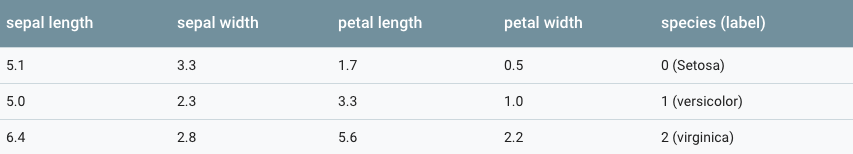
\includegraphics[\textwidth]{images/table}
  \caption{Data representation used for modeling (taken from~\cite{tensor18})}
  \label{fig: rep}
\end{figure}

Although TensorFlow Linear Classifier Estimator was also applicable for this problem, it was required to use the DNNClassifier to perform multi-class classification~\cite{tensor18}. Because the information volume was not very large it was appropriate to develop a four layer model. The two outer layers correspond to the indispensable input and output layers, as a result  two hidden layers remained in the net. Specifically entering into details concerning the Neural Network development, the DNNClassifier  provided accesible tools to model the net.

\begin{tensorflow}[caption={ads}]
# Net contains 2 hidden layers with 10 nodes each.
classifier = tf.estimator.DNNClassifier(
    feature_columns=my_feature_columns,
    hidden_units=[10, 10],
# The model must choose between 3 classes which represent each flower.
    n_classes=3)
\end{tensorflow}

Continuing with the model development, as implemented in the project above, the first steps to achieve a good model was creating the input functions, and defining the model's feature columns. 

\begin{tensorflow}[caption={ads}]
#Input function definition
def input_evaluation_set():
    features = {'SepalLength': np.array([6.7, 5.3, 4.4]),
                'SepalWidth':  np.array([3.4., 4.2, 3.1]),
                'PetalLength': np.array([5.6, 3.3, 4.8]),
                'PetalWidth':  np.array([2.2, 1.0, 2.8])}
    labels = np.array([3, 1])
    return features, labels
\end{tensorflow}

Interestingly the results obtained by the model's classification where expected to sum up to one. In other words, the model was designed to respond to each input by deciding in which proportion the data corresponds to one of the three available flowers. 

\begin{enumerate}
 \item 0.08 for Iris Setosa
 \item 0.02 for Iris Versicolor
 \item 0.90 for Iris Virginica
\end{enumerate}

From the above example it is possible to conclude that the model determined a 90 percent probability of the data corresponding to an Iris Virginica.   Following this, the closing section of the process was developed in a similar manner to the first project. Namely, training the model and evaluating proceeded. Just like in the first  application, training was implemented using the Estimators train method. 

%%%%
\subsection{Experiments Analysis}
\authorcomment[missing]{}{Why is better to to linear regression than neural networks for supervised learning applications, and viceversa}

For both the Housing and Flower problems models were trained and predictions were made.  From here evaluations were made concluding that indeed linear regression models present useful solutions while keeping things simple. 

The second project developed with data and guidance provided by TensorFlow where the main goal was to classify flowers based on a dataset containing plant measurements such as sepal length, sepal width, petal length and petal width. The Model had to classify the data into one of three iris flowers: Iris setosa, Iris versicolor and Iris virginica.  As said before in this document, it was necessary to set a representation of these classifications for the model to work. Contrary to the method implemented in the first project (supervised machine learning with linear regression) to solve this problem a Deep Neural Network model was implemented. 


%%%%
\subsection{Threads to Validity}



\endinput




% $  Id: conclusion.tex  $
% !TEX root = main.tex

%%
\section{Conclusion}
\label{sec:conclusion}

This paper offers a perspective on the wide subject of \ac{AI} and \ac{ML}. The purpose of the paper 
is disambiguate the purpose and use of \ac{ML} approaches for software development. In particular 
we focus on the question of what is the best technique for pattern recognition based on a given 
dataset. We explored the six existing approaches in \ac{ML}. The paper presents an empirical 
validation for the two approaches that exhibited the most promising results for the problem at hand, 
supervised learning and deep learning. The linear regression technique among the supervised 
learning approaches is identified as the most suitable technique for pattern recognition. Nonetheless, 
\acl{NN} also provide satisfactory results in patters classification. 
To conduct our experiments we use the TensorFlow Estimator API and the column-oriented data 
analysis API Pandas. We highlight the fact that the use of this frameworks eases the learning curve 
to \ac{ML}, and the start of a new \ac{ML} project.

As part of our future work, we would like to extend our empirical study in three directions. First we 
would like to cover all six sub-categories of \ac{ML}. Second, we would explore other application 
domains, different to pattern recognition. Finally, we would like to use the experiment to compare 
different frameworks realizing \ac{ML}, such as the Amazon AWS, or Artificial Neural Networks. 
As a final goal of this project we would like to build a characterization and a compendium of projects 
that are suitable for the use of \ac{ML}, and which one are not.

\endinput




%
%\balancecolumns

%\printbibliography
\bibliographystyle{splncs03}
\bibliography{local,bib/compsci,bib/general,bib/learning,bib/collabide}  


\end{document}

